\documentclass{article} % Tipo de documento

\usepackage[utf8]{inputenc} % Permite el uso de caracteres del Español

\usepackage[T1]{fontenc}
\usepackage{graphicx}
\usepackage{float}

% Carátula del Artículo

\title{Atmosfera Terrestre}

\author{Ramses Pacheco}

\date{30 de Enero, 2018}



% Comentario invisible



\begin{document}

\maketitle % Crea el título

\section{composición}

La atmósfera de la tierra  rige las leyes de los gases ,la atmósfera terrestre protege la vida en la tierra creando una cierta presión que hace que exista agua liquida en la superficie de la tierra y reduciendo la temperatura extrema entre el dia y la noche.
el aire seco por volumen contiene 78\% de nitrógeno,20.95\% de oxigeno,0.93\% de argón,0.04\% de dióxido de carbono y otras pequeñas cantidades de gases.El contenido de aire y la presión atmosférica varían en las diferentes capas.

Los tres componentes principales del aire, y por lo tanto de la atmósfera de la Tierra, son nitrógeno, oxígeno y argón. El vapor de agua representa aproximadamente el 0,25\% de la atmósfera en masa. La concentración de vapor de agua.Muchas sustancias de origen natural pueden estar presentes en pequeñas cantidades y comúnmente en variables como aerosoles.

\section{Estructura de la atmósfera}
\subsection{capas principales}

En general la presión del aire y la densidad decrecen con la altitud en la atmósfera. Sin embargo la temperatura del aire es mas complicada en las alturas,y puede permanecer relativamente constante o incluso aumentar con la altitud en algunas regiones. De esta manera, la atmósfera de la Tierra se puede dividir en cinco capas principales:

\subsubsection{Exosfera}
la exosfera y la capa mas exterior de la atmosfera terrestre,se extiende desde la exobase, que se encuentra en la parte superior de la termosfera a una altitud de aproximadamente 700 km sobre el nivel del mar, a unos $10,000$ km, donde se funde el viento solar.

Esta capa está compuesta principalmente de densidades extremadamente bajas de hidrógeno, helio y varias moléculas más pesadas, incluyendo nitrógeno, oxígeno y dióxido de carbono más cerca de la exobase. Los átomos y las moléculas están tan separados que pueden viajar cientos de kilómetros sin colisionar entre sí.
En la exosfera, las partículas escapan constantemente al espacio. Estas partículas que se mueven libremente siguen trayectorias balísticas y pueden migrar dentro y fuera de la magnetosfera o del viento solar.
Sin embargo, la aurora boreal y la aurora austral a veces se ocurren en la parte inferior de la exosfera, donde se superponen a la termosfera. La exosfera contiene la mayoría de los satélites que orbitan alrededor de la Tierra.

\subsubsection{Termosfera}
La termosfera es la segunda capa mas alta de la atmosfera terrestre.se extiende desde la mesopausa a una altitud aproximadamente 80 km arriba de la termopausa La altura de la termopausa varía considerablemente debido a los cambios en la actividad solar.La parte inferior de la termosfera, de 80 a 550 kilómetros sobre la superficie de la tierra, contiene la ionosfera.

La temperatura de la termosfera decrece conforme la altura,porque a diferencia a la estratosfera debajo de ella en donde una inversión de temperatura se debe a la absorción de radiación por el ozono.

La temperatura de esta capa puede elevarse hasta $1500^\circ$C.
La termosfera tiene una alta cantidad de moléculas con alta energía,
no estaría caliente para un humano ya que la densidad de las moléculas son muy bajas para conducir una cantidad de energía considerable.
\subsubsection{Mesosfera}
la mesosfera es la tercera capa mas alta de la atmósfera de la tierra,Se extiende desde la estratopausa a una altitud de aproximadamente 50 km a la mesopausa a 80-85 km sobre el nivel del mar.Las temperaturas descienden con el aumento de altitud hacia la mesopausa,que marca la parte superior de esta capa media de la atmósfera. Es el lugar más frío de la Tierra y tiene una temperatura promedio de alrededor de $-85^\circ$C,
la mesosfera es tambien la capa donde la mayoria de los meteoros se queman al entrar en la atmosfera.

\subsubsection{Estratosfera}
La estratosfera es la segunda capa más baja de la atmósfera de la Tierra.Esta capa se extiende desde la parte superior de la troposfera a aproximadamente 12 km de la superficie de la Tierra hasta la estratopausa a una altitud de aproximadamente 50 a 55 km.

\begin{figure}[ht!]
  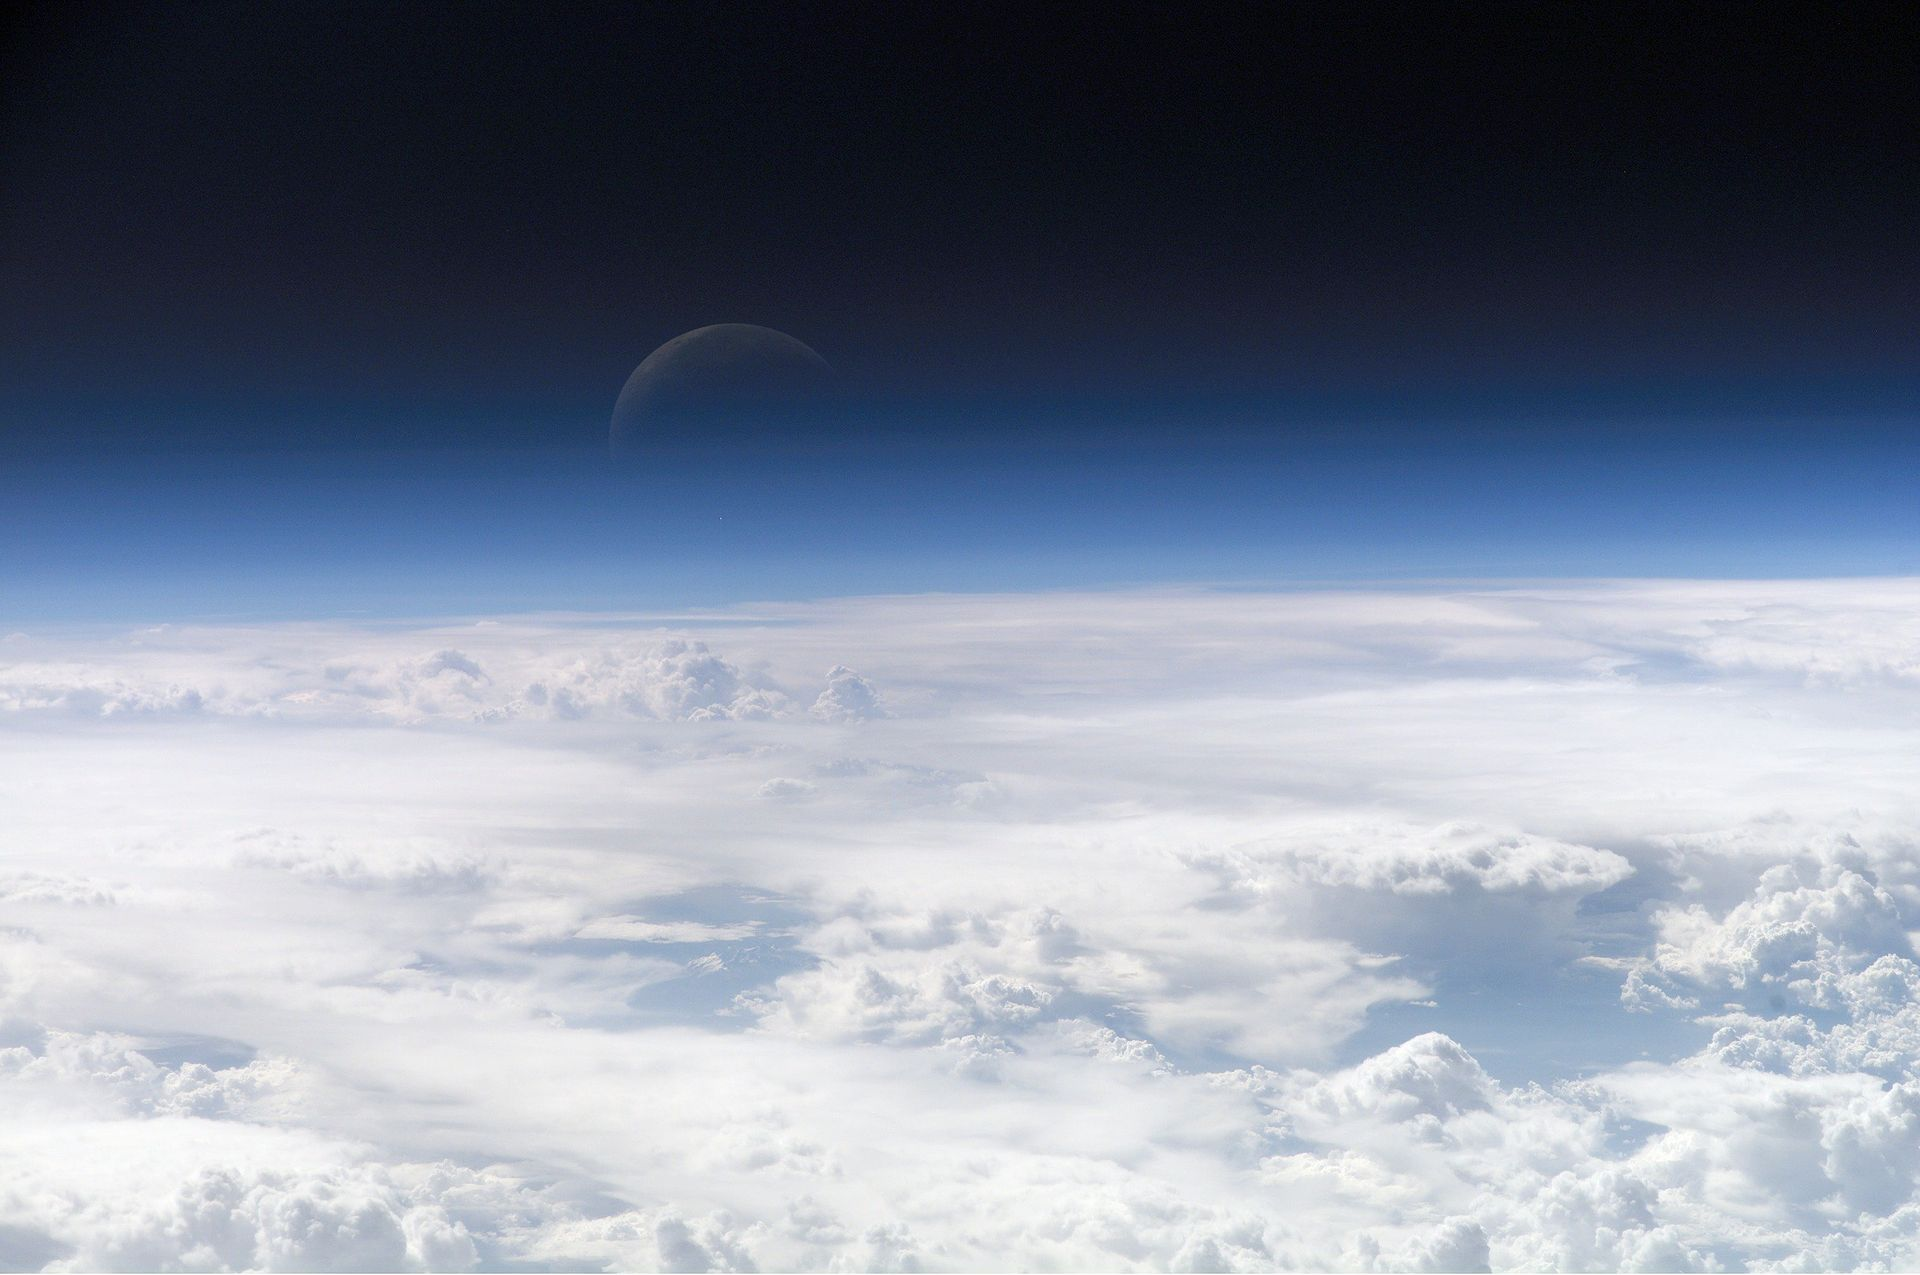
\includegraphics[width=\linewidth]{cielo.jpg}
  \caption{Imágen CC: NASA (Wikimedia Commons).}
  \label{fig:cielo1}
\end{figure}

La presión atmosférica en la parte superior de la estratosfera es aproximadamente 1/1000 de la presión al nivel del mar. La estratosfera define una capa en la que las temperaturas aumentan con el aumento de la altitud.Este aumento de la temperatura es causado por la absorción de la radiación de rayos ultravioleta por la capa de ozono.

\subsubsection{troposfera}
 La troposfera está delimitada por encima por la tropopausa, un límite marcado en la mayoría de los lugares por una inversión de temperatura (es decir, una capa de aire relativamente cálido por encima de uno más frío).

La troposfera contiene aproximadamente el 80\% de la masa de la atmósfera terrestre.La troposfera es más densa que todas las capas atmosféricas que la recubren porque un peso atmosférico más grande se encuentra en la parte superior de la troposfera y hace que se comprima más severamente.

 Básicamente tiene todos los tipos de nubes nubladas asociadas al clima generadas por la circulación activa del viento,la actividad de aviación más convencional tiene lugar en la troposfera, y es la única capa a la que se puede acceder mediante un avión propulsado por hélice.

\subsubsection{otras capas}

Una de las principales capas secundarias es la ionosfera es una región de la atmósfera ionizada por la radiación solar. Es responsable de auroras. Durante el día, se extiende de 50 a 1,000 km, e incluye la mesosfera, la termosfera y partes de la exosfera.

La homósfera y la heterosfera se definen según si los gases atmosféricos están bien mezclados. La homosfera basada en la superficie incluye la troposfera, la estratosfera, la mesosfera y la parte más baja de la termosfera y la  composición química de la atmósfera no depende del peso molecular por la turbulencia.

Sobre esta altitud se encuentra la heterosfera, que incluye la exosfera y la mayor parte de la termosfera. Aquí, la composición química varía con la altitud.

La capa límite planetaria es la parte de la troposfera más cercana a la superficie de la Tierra y directamente afectada por ella, principalmente a través de la difusión turbulenta. Durante el día, la capa límite planetaria suele estar bien mezclada, mientras que por la noche se estratifica de manera estable con una mezcla débil o intermitente.

\begin{figure}[ht!]
  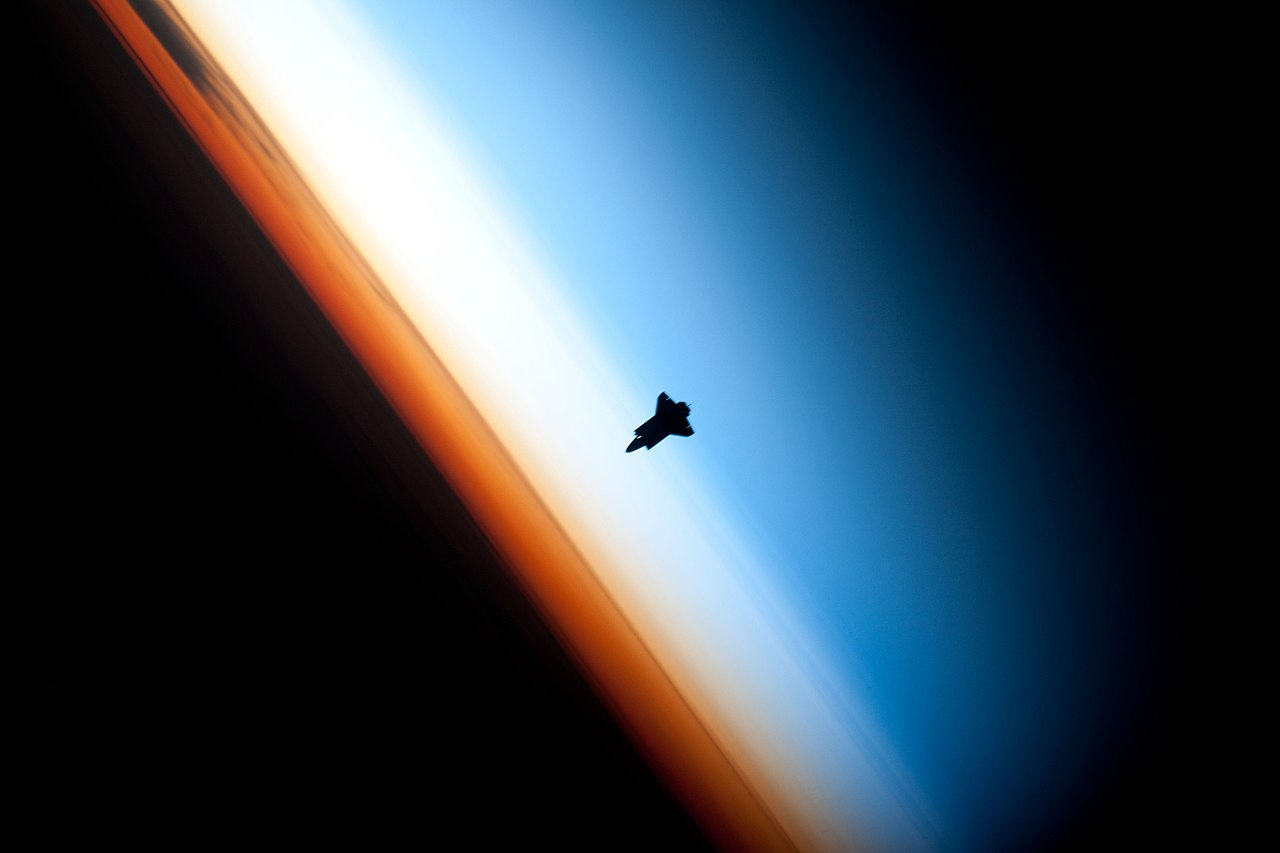
\includegraphics[width=\linewidth]{cielo2.jpg}
  \caption{Imágen CC:colores de horizontes de la tierra(wikimedia commons)}
  \label{fig:cielo2}
\end{figure}



\section{Propiedades físicas}
\subsection{Presión y densidad}
La presión atmosférica promedio a nivel del mar está definida por la Atmósfera Estándar Internacional como 101325 pascales(atm).
Si toda la masa de la atmósfera tuviera una densidad uniforme desde el nivel del mar, terminaría abruptamente a una altitud de 8,50 km. En realidad, disminuye exponencialmente con la altitud, disminuyendo a la mitad cada 5,6 km (18,000 pies) o por un factor de 1 cada cada 7,64 km.

Las diversas capas de la ionosfera de la Tierra, importantes para la propagación de la radio en ondas decamétricas, comienzan a menos de 100 km y se extienden más allá de 500 km.Dependiendo de la actividad solar, los satélites pueden experimentar una resistencia atmosférica notable a altitudes de hasta 700-800 km.

\subsection{temperatura y velocidad del sonido}
La temperatura disminuye con la altitud comenzando al nivel del mar, pero las variaciones en esta tendencia comienzan por encima de los 11 km, donde la temperatura se estabiliza a través de una gran distancia vertical a través del resto de la troposfera.
La velocidad del sonido depende únicamente de la temperatura y no de la presión o densidad del gas,la velocidad del sonido en la atmósfera con la altitud adquiere la forma del perfil de temperatura complicado  y no refleja los cambios altitudinales en densidad o presión.


\subsection{Densidad y masa}
La densidad del aire a nivel del mar es de aproximadamente 1.2 kg/m$^{3}$, la densidad no se mide directamente, pero se calcula a partir de mediciones de temperatura, presión y humedad utilizando la ecuación de estado para el aire.

La masa promedio de la atmósfera es de aproximadamente 5 cuatrillones,La masa media total de la atmósfera es 5.1480$\times ^{algo}$ kg con un rango anual debido al vapor de agua de 1.2 o 1.5$\times ^{algo}$ kg, dependiendo de si se usan datos de presión superficial o vapor de agua algo más pequeña que la estimación anterior.

\section{propiedades ópticas}
La radiación solar,es la energía que recibe la Tierra del sol. La Tierra también emite radiación hacia el espacio, pero a longitudes de onda más largas que no podemos ver.
\subsection{Dispersión}
cuando la luz pasa a través de la atmósfera de la tierra ,los fotones interactúan con ella a través de la dispersión. si la luz no, interactúa con la atmósfera se le llama radiación directa, la radiación indirecta es la luz que se ha dispersado en la atmósfera.Por ejemplo, en un día nublado cuando no puedes ver tu sombra no hay radiación directa que te llegue, todo se ha dispersado.
\subsection{Absorción}
Diferentes moléculas absorben diferentes longitudes de onda de radiación.
Los espectros de absorción combinados de los gases en la atmósfera dejan "ventanas" de baja opacidad, permitiendo la transmisión de solo ciertas bandas de luz.
\subsection{Emisión}
La emisión es lo opuesto a la absorción, es cuando un objeto emite radiación,los objetos más calientes tienden a emitir más radiación, con longitudes de onda más cortas. Los objetos más fríos emiten menos radiación, con longitudes de onda más largas.
Debido a su temperatura, la atmósfera emite radiación infrarroja. Por ejemplo, en las noches despejadas, la superficie de la Tierra se enfría más rápido que en las noches nubladas.

\subsection{Indice de refracción}
El índice de refracción del aire es cercano, pero apenas superior a 1. Las variaciones sistemáticas en el índice de refracción pueden conducir a la flexión de los rayos de luz en recorridos ópticos largos.

\section{Circulación}
La circulación atmosférica es el movimiento de aire a gran escala a través de la troposfera, y los medios,con circulación oceánica por los cuales se distribuye el calor alrededor de la Tierra.


\begin{figure}[ht!]
  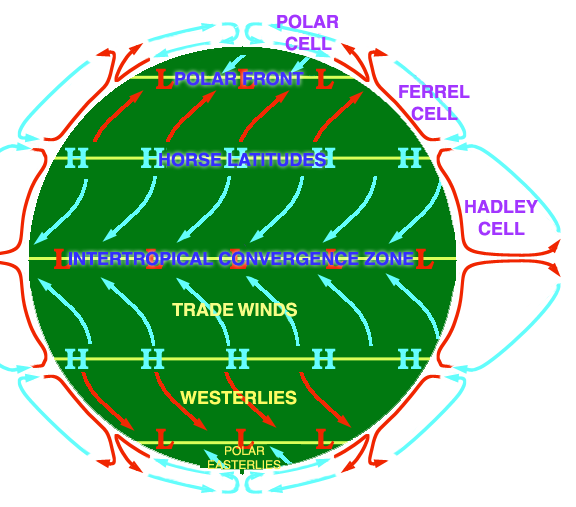
\includegraphics[width=\linewidth]{cielo5.png}
  \caption{Imágen CC:circulación(wikimedia commons)}
  \label{fig:cielo5}
\end{figure}




\section{Apéndice}
1.-¿Qué fue lo que más te llamó la atención de esta actividad?

Se me hizo muy interesante la forma en que podemos cambiar las letras y lo fácil que es,y que es muy similar a un tipo de programación,pero mas sencillo,con mas herramientas accesibles.


2.-¿Qué fue lo que se te hizo menos interesante?
La verdad,no hay ninguna cosa en que no me haya interesado,ya que es un nuevo programa para mi y me gusto mucho su funcionamiento y sus herramientas


3.-¿Qué cambios harías para mejorar esta actividad?
Talvéz, explorar un poco mas las herramientas como insertar ecuaciones,diferentes tipos de estructura del documento a crear,realizar diagramas,etc.


4.-¿Cuál es tu primera impresión de uso de LATEX?
Excelente ya que es una herramienta fantástica, que te facilita mucho las cosas para cuestiones matemáticas,reportes,ensayos ,etc.


5.-¿El tiempo sugerido para esta actividad fue suficiente?
si,fue suficiente


6.-¿Encontraste algún documento o recurso en línea útil que quisieras compartir con los demás?
No encontré algo mas fuera de lo normal.




\section{Bibliografía}

wikipedia,29 de marzo del 2003,\textit{Atmosfera terrestre}












\end{document}



